\section{Unity}
Unity нь видео тоглоом, симуляци болон бусад интерактив контентыг үүсгэх, хөгжүүлэхэд ашигладаг cross-platform тоглоомын engine юм. Уг тоглоомын engine нь физик, график, скрипт, нөөцийн менежмент гэх мэт тоглоом хөгжүүлэх олон төрлийн хэрэгсэл, функцээр хангадаг.
\subsection{Scene}
Unity-д Scene нь тоглоомын программын элементүүдийн агуулах ба үүнд GameObjects, гэрэлтүүлэг, камерын тохиргоо болон бусад нөөц орно . Scene-г тоглоомын бие даасан хэсэг эсвэл үе гэж үзэж болох бөгөөд олон Scene-г нэг доор ажиллуулж болдог. Scene-үүдийг динамикаар ачаалж, буулгах боломжтой.
\subsection{GameObject}
Unity-д GameObject нь үзэгдэл дэх тоглоомын объектыг төлөөлөх үндсэн объект юм. GameObject-нь үүнд гол үүрэг, зан чанарыг тодорхойлдог Component-уудын агуулах юм.
\subsection{Component}
Component нь Unity дахь GameObject-д тодорхой функцүүдийг өгдөг модульчлагдсан кодын хэсэг юм. Component-д скрипт, физикийн коллайдерууд, моделийн материалууд орно. GameObject-ийн үйлдлийг өөрчлөхийн тулд бүрэлдэхүүн хэсгүүдийг нэмж, устгаж, өөрчилж болно.
\subsection{Prefab}
Prefab нь GameObject болон түүнтэй холбоотой component-уудыг агуулсан дахин ашиглах боломжтой нөөц бөгөөд Scene-д олон удаа үүсгэж болно. Prefab-ууд нь хөгжүүлэгчдэд объектыг нэг удаа  үүсгэж, тоглоом эсвэл программынхаа туршид дахин ашиглах боломжийг олгодог.
\subsection{ScriptableObject}
Unity дээр өөр дахин ашиглах боломжтой нөөц ба энэ нь Prefab-с Scene-с гадуур ашиглагдаж чаддагаараа өөр.
\subsection{MonoBehaviour болон үүний амьдралын мөчлөг}
MonoBehaviour нь скриптүүдийг Unity engine-тэй харилцах боломжийг олгодог component юм. Component-н функциональ зан чанарыг тодорхойлоход ашиглаж болох Start(), Update() болон OnTriggerEnter() зэрэг функцүүдээр хангадаг.
Амьдралын мөчлөгийг \ref{fig:MonoBehaviourFlowChart1} үзүүлэв.
\begin{figure}[t]
	\centering
	\caption{MonoBehaviour амьдралын мөчлөг эхний хэсэг}
	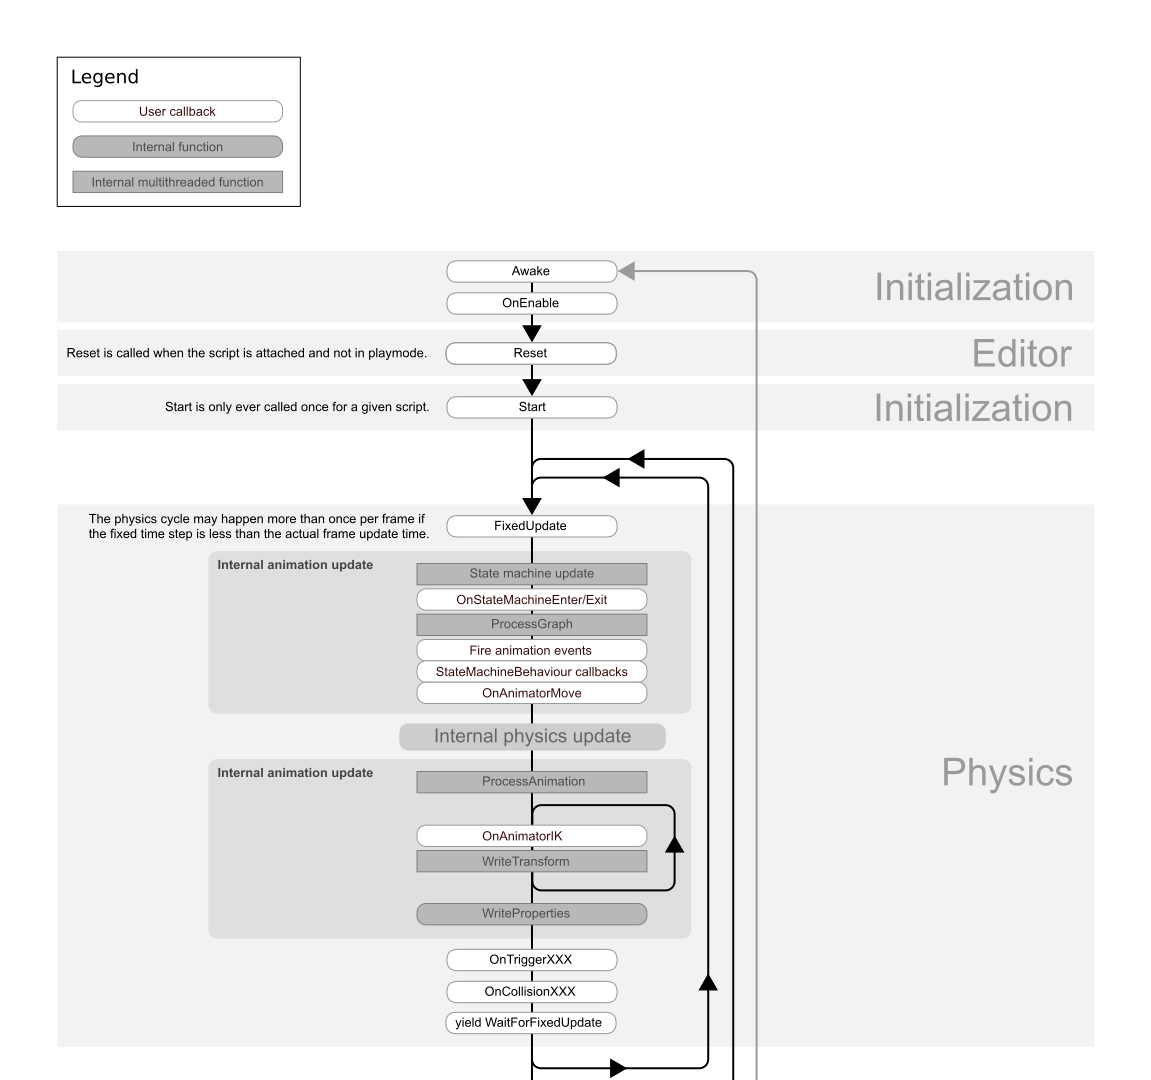
\includegraphics[width=\textwidth]{./images/monobehaviour_flowchart_1.png}
	\label{fig:MonoBehaviourFlowChart1}
\end{figure}
\begin{figure}[b]
	\centering
	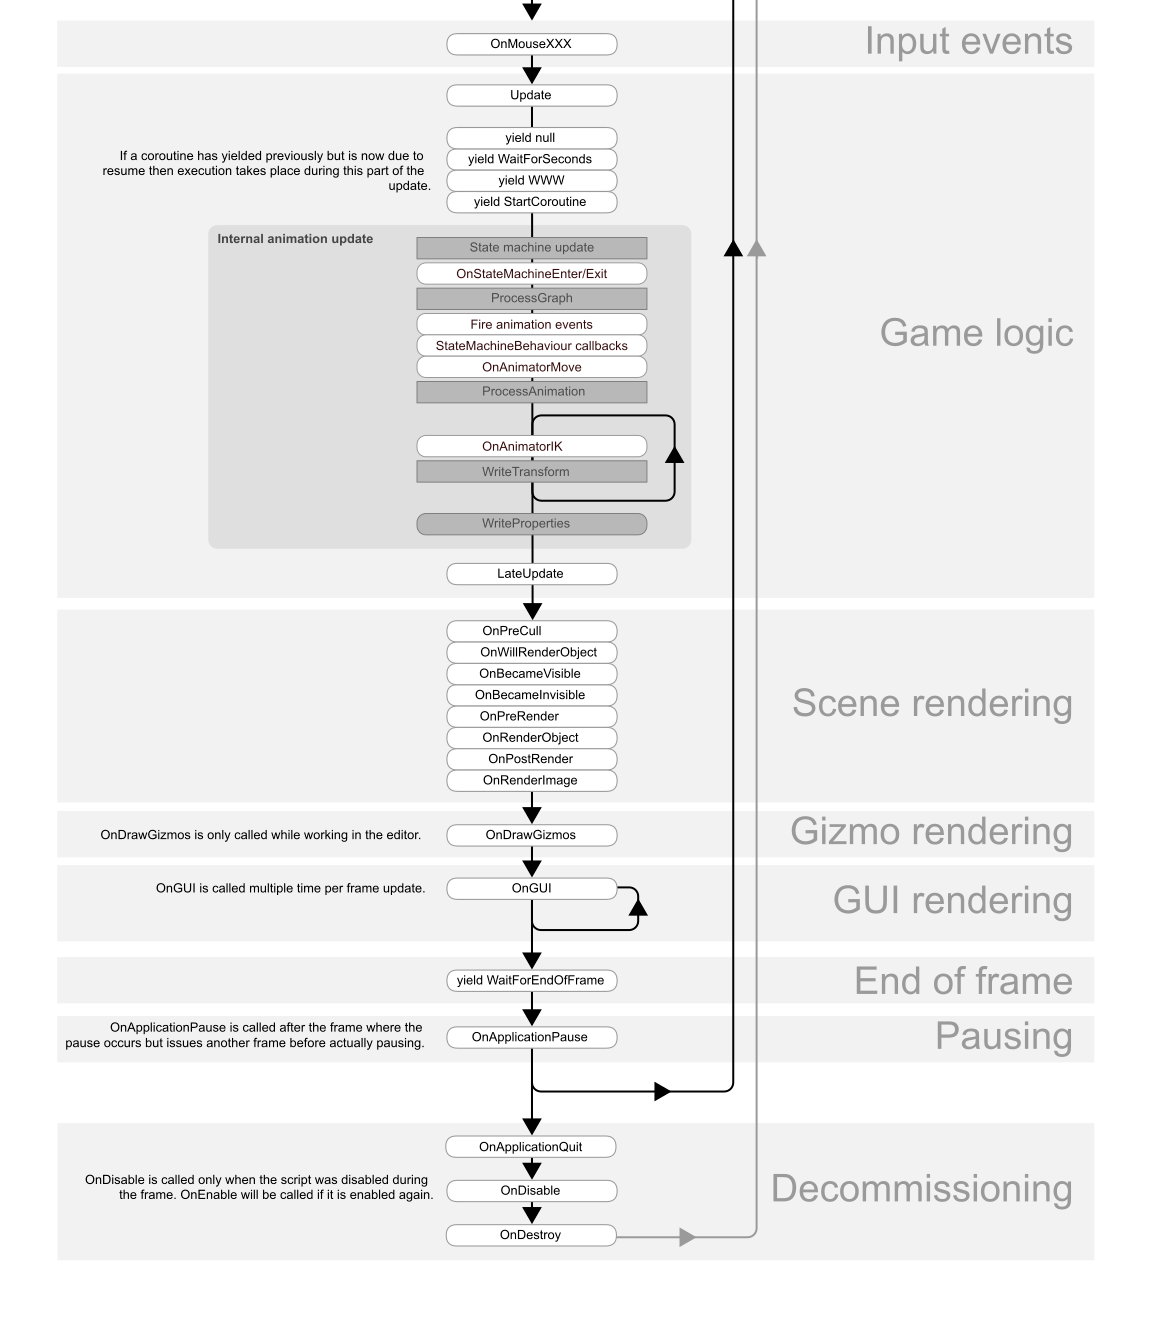
\includegraphics[width=\textwidth]{./images/monobehaviour_flowchart_2.png}
	\caption{MonoBehaviour амьдралын мөчлөг хоёр дахь хэсэг}
	\label{fig:MonoBehaviourFlowChart2}
\end{figure}


\subsection{ProBuilder}
Unity дээр моделийг үүсгэх, өөрчлөх мөн тоглоомыг үеийг засварлах хэрэгсэл.
\section{C\#}
Кодын хэл ба Unity дээр Component-г тодорхойлоход ашиглана.
\section{IntelliJ Rider}
Unity-тэй сайн холболттой. Код highlighting, refactoring, debugging, completion зэрэг функцуудтай IDE.
\section{PlasticSCM}
Тоглоомын төслийн хөгжүүлэлтэд нийтлэг ашиглагддаг Version Control хэрэгсэл. Нийтлэг branching, merging, code reviews зэрэг version control хэрэгслүүдийн функционалийг агуулдаг. Харин PlasticSCM нь бусад version control-тэй харьцуулахад том файлуудтай болон тоглоомын хөгжүүлэлтийн нөөцүүдтэй харьцахад илүү амар.
